\documentclass[10pt]{exam}
\usepackage[utf8]{inputenc}

\usepackage[margin=1in]{geometry}
\usepackage{amsmath,amssymb}
\usepackage{multicol}
\usepackage{multirow}
\usepackage{graphicx}
\usepackage{tikz}
\newcommand{\clase}{CÁLCULO INTEGRAL}
\newcommand{\examnum}{Parcial 1}
\newcommand{\examdate}{21 de Febrero de 2020}
\newcommand{\timelimit}{120 Minutos}
\definecolor{Micolor1}{gray}{0.7}
\pagestyle{head}
\firstpageheader{\Large\sc\clase}{}{\sc\examnum}
\runningheader{\sc\clase}{}{\sc\examnum\ - Page \thepage\ of \numpages}
\runningheadrule


\begin{document}
\vspace{1.5cm}
\begin{tabular}{ll}
\multirow{5}{*}{
\includegraphics[scale=0.28]{Sabana1.png}}
%&\textbf{Examen Final}\\
& \large\hspace{0.5cm}Nombre: \makebox[2.7in]{\hrulefill}\vspace{0.2cm}\\
& \large\hspace{0.5cm}Fecha:\textbf{\examdate} \vspace{0.2cm}\\
& \large\hspace{0.5cm}Tema: B \vspace{0.2cm}\\
& \large\hspace{0.5cm}Profesor: \makebox[2.7in]{\hrulefill}\vspace{0.2cm}\\
%& \large\hspace{1.0cm}Tiempo límite: \textbf{\timelimit}}
\end{tabular}\\
\rule[2ex]{\textwidth}{2pt} 
\begin{itemize}
\scriptsize{\item \textbf{No se permite el uso de elementos electrónicos, smartwatches, etc. La presencia de cualquier equipo de comunicación en el entorno del examen es considerado intento de fraude. Éste o cualquier otro intento de fraude implica cero en el examen y se reporta a la facultad.}
    \item \textbf{La comprensión del examen es parte de la evaluación, por tanto, no se responden preguntas.} 
    \item \textbf{Se evalúa procedimiento y/o justificación, por tanto, sea claro y ordenado.}
   % \item \textbf{Este examen contiene \numpages\ páginas y \numquestions\ preguntas.  El Total de puntos en esta prueba es de \numpoints}
   }
\end{itemize} 

%\begin{center}
%\textbf{Tabla de Puntos (No marcar. Uso exclusivo del profesor)}\\
\addpoints
%\gradetable[v][questions]
%\end{center}

\noindent
\rule[2ex]{\textwidth}{2pt}


\begin{enumerate}
\normalsize
\setlength{\columnsep}{10mm}


   \item El tamaño de una población en condiciones ideales varía a una tasa de: $$P'(t)=\frac{2t}{t^2+1}+e^{-3t},\,\,\,\,\text{miles de personas/año}$$
 \begin{enumerate}

    \item \textbf{[4 puntos]} ¿Se puede afirmar que el tamaño de la población aumenta con el tiempo? Justifique \hfill{[B1]}
     \item \textbf{[8 puntos]} Calcule la funci\'on $P(x)$ que representa el tamaño de la poblaci\'on. \hfill{[B2]}
   %  \item \textbf{[4 puntos]} Si el recipiente está totalmente lleno y empieza a salir agua a una velocidad de $\dfrac{}{}$ tomamos la constante de integraci\'on igual a cero, tiene sentido el valor $P(0)$. Justifique en palabras. \hfill{[B3]} 
 \end{enumerate}


   \item \textbf{[4 puntos]} Calcule $$\int \left(x^2 + \cos(a)+\dfrac{1}{x}+\dfrac{1}{a^2}\right)\, dx$$ 

donde $a$ es una constante positiva. \hfill{[C1]} 


\item El costo total $C(x)$ (en dólares) por la compra y el mantenimiento de la pieza de una máquina durante $x$ años está dado por

\[C(x)=1000\left(20+3\int_0^x t^{1/2} dt\right)\]


\begin{enumerate}
    \item  \textbf{[4 puntos]} ¿Cuál es fue el costo inicial de la pieza?\hfill{[B3]}
    \item  \textbf{[4 puntos]} ¿Cuál es el costo total de la pieza en el primer año de uso?\hfill{[B1]}
    \item \textbf{[8 puntos]} ¿Cuál es el costo marginal en el primer año de uso? \hfill{[B2]}



\end{enumerate}

  
\item \textbf{Assist Ingeniería S.A.S} planea fabricar un recipiente en forma de bala para almacenar agua. Para su fabricación, rotará alrededor del eje $x$ la región sombreada en la figura.

\begin{center}
    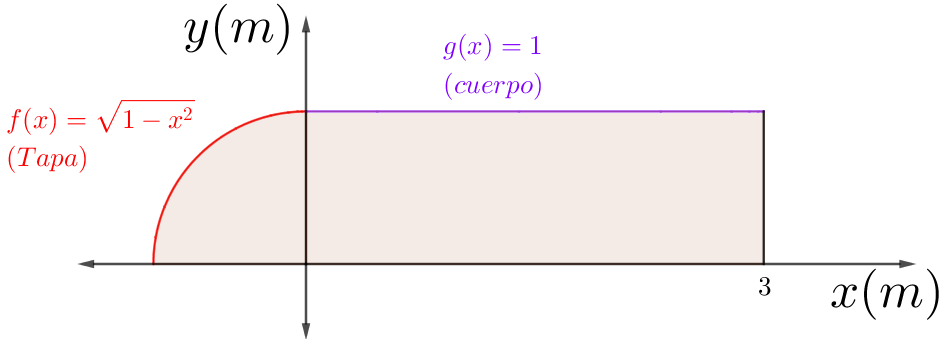
\includegraphics[scale=1.5]{Depositobala2.png}
\end{center}

\begin{enumerate}
   \item \textbf{[6 puntos]} Plantee la integral que represente el volumen de la tapa de la bala (rotación de $f(x)$). \hfill{[B2]}

   \item \textbf{[6 puntos]} Plantee la integral que represente el volumen del cuerpo de la bala (rotación de $g(x)$). \hfill{[B2]}
    
   \item \textbf{[4 puntos]} Si el recipiente está completamente lleno y empieza a salir agua a una velocidad de $\pi\,m^3/h$.  ¿Cuánto tiempo demora en desocuparse el tanque?  \hfill{[B3]}
    
    
\end{enumerate}

\item Las siguientes gráficas representan una aproximación y el área, de la región bajo la curva $f(x)=x^2+\dfrac{1}{2}$ desde $x=-2$ hasta $x=1$.

\begin{center}
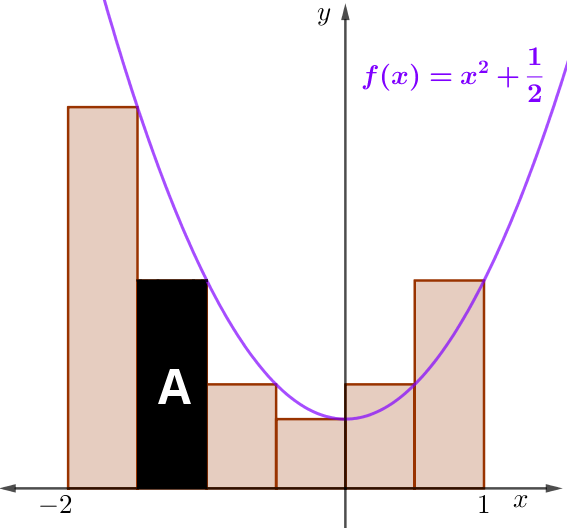
\includegraphics[scale=1.2]{Riemann6.png}
\hspace{0.5 cm}
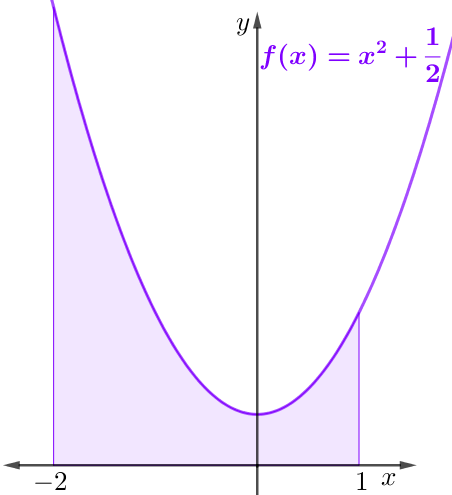
\includegraphics[scale=1.2]{R3.png}    
\end{center}

\begin{enumerate}
    \item \textbf{[4 puntos]} Calcule el área del rectángulo marcado con la letra A. \hfill{[C1]}
    \item \textbf{[8 puntos]} Calcule la suma de las áreas de los rectángulos de aproximación de la figura izquierda, (la partición es regular, es decir, todos los rectángulos tienen la misma base). \hfill{[C2]}
    \item \textbf{[8 puntos]} Calcule el área de la región sombreada de la figura derecha. \hfill{[C1]}

    \item \textbf{[4 puntos]}Al calcular el área bajo la curva, ¿cuál es el error de aproximación que se comete en la figura izquierda?  \hfill{[C3]}


\end{enumerate}

\item Un fabricante de neumáticos estima que los mayoristas comprarán (demandarán) $q$ (miles) de neumáticos radiales cuando el precio sea $$p=-q^2-q+6,\,\,\,\,\,\,\, q>0$$
dólares por neumático, y el mismo número de neumáticos se ofertarán cuando el precio sea $$p=4q$$
dólares por neumático.

\begin{enumerate}
    \item \textbf{[4 puntos]} Encuente el punto de equilibrio del mercado. \hfill{[C2]}
    
    \item \textbf{[8 puntos]} ¿Cuál es el excedente del productor del mercado? \hfill{[C2]}
\end{enumerate}

\end{enumerate}





\end{document}
